\documentclass{cssheet}

%--------------------------------------------------------------------------------------------------------------
% Basic meta data
%--------------------------------------------------------------------------------------------------------------

\title{Verkettung von zwei Achsenspiegelungen}
\author{Prof. Dr. Christian Spannagel}
\date{\today}
\hypersetup{%
    pdfauthor={\theauthor},%
    pdftitle={\thetitle},%
    pdfsubject={Aufgabenblatt Geometrie},%
    pdfkeywords={geometrie}
}


%--------------------------------------------------------------------------------------------------------------
% document
%--------------------------------------------------------------------------------------------------------------

\begin{document}
\printtitle

In den nächsten Wochen werden wir mehrere Kongruenzabbildungen hintereinander ausführen. Das heißt, dass wir die Abbildungen \emph{verketten}. Man schreibt $f\circ g$. Der Einfachheit halber führen wir die Abbildungen auch von links nach rechts aus, d.\,h. erst wird die Abbildung $f$ ausgeführt, dann die Abbildung $g$. (Das ist anders, als man es etwa aus dem Bereich der reellen Funktionen gewöhnt ist.)
 
In diesem Aufgabenblatt untersucht ihr, welche Abbildung sich ergibt, wenn man nacheinander an zwei Achsen $f$ und $g$ spiegelt. 

\textbf{Aufgabe 1 (Kopunktale Achsen):}  Gegeben seien zwei Geraden $f$ und $g$, die sich im Punkt $S$ im Winkel $\alpha$ schneiden.
\begin{center}
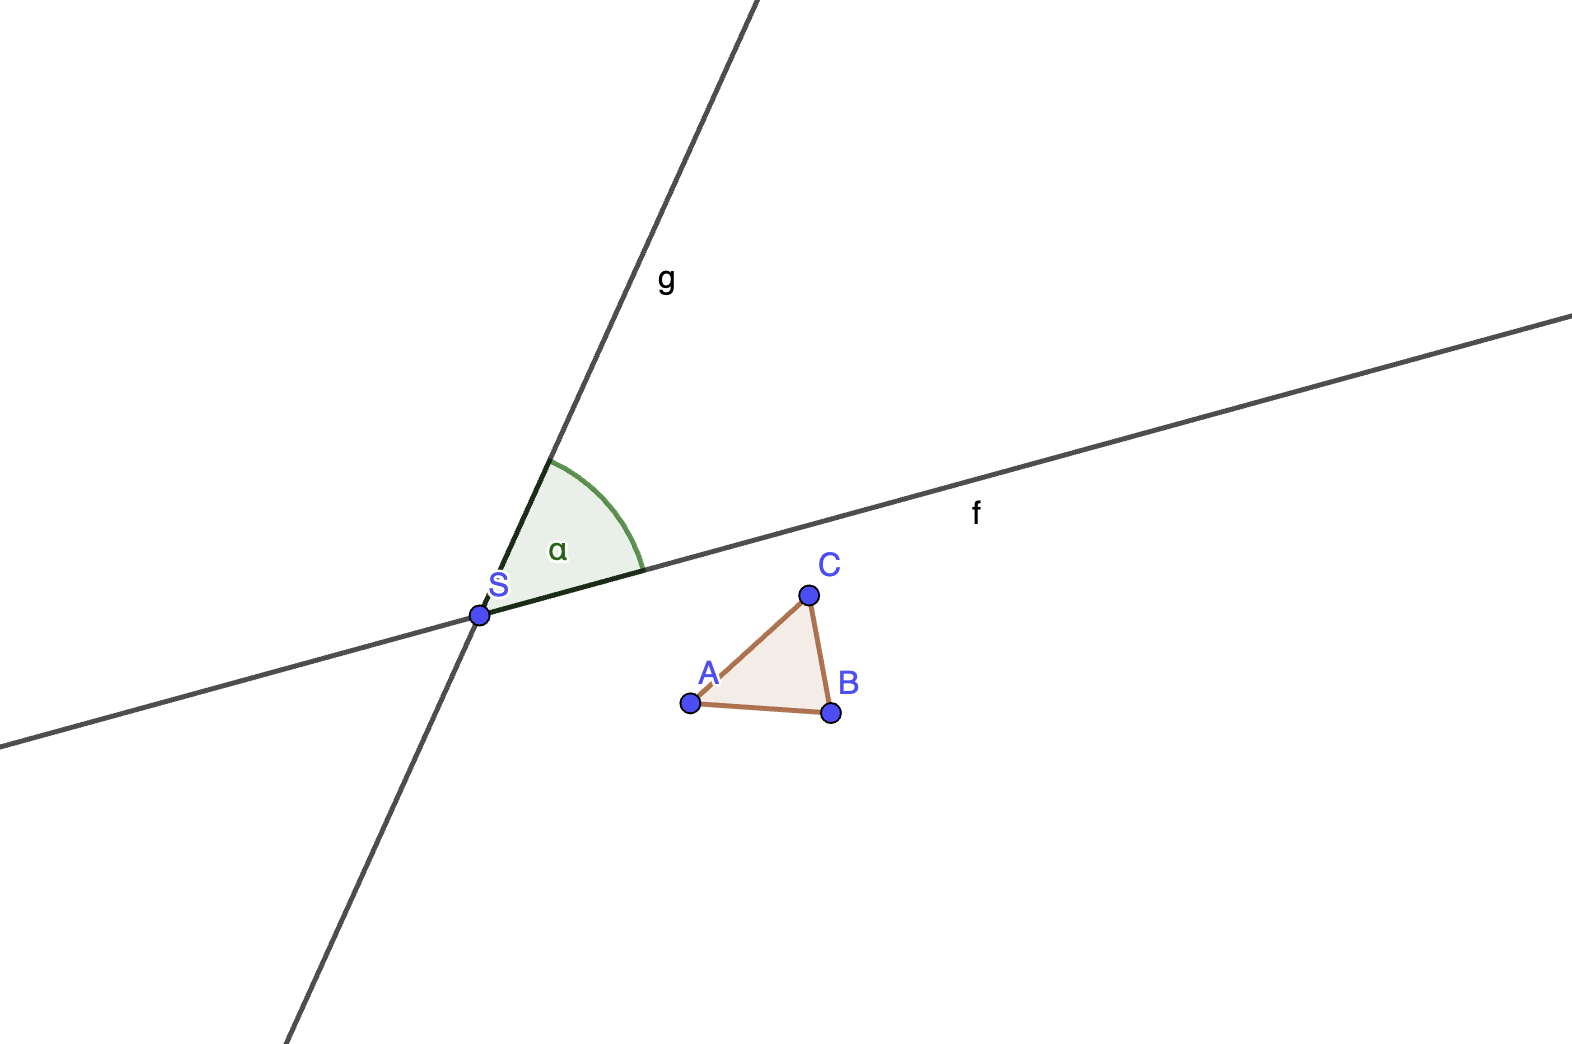
\includegraphics[width=10cm]{sich-schneidende-geraden.png}
\end{center}
\begin{enumerate}[a)]
\item Spiegelt ein allgemeines Dreieck nacheinander an den beiden Geraden in Geogebra. 
\item Dreht die Geradenkreuzung bei festem Winkel $\alpha$ um $S$. Was passiert? Könnt ihr euch das erklären?
\item Welche Abbildung ist $f\circ g$? Charakterisiert die Abbildung möglichst genau unter Verwendung von $S$ und $\alpha$. Begründet, warum es sich um diese Abbildung handelt.
\end{enumerate}

\textbf{Aufgabe 2 (Parallele Achsen):}  Gegeben seien zwei parallele Geraden $f$ und $g$ mit Abstand $d$.
\begin{center}
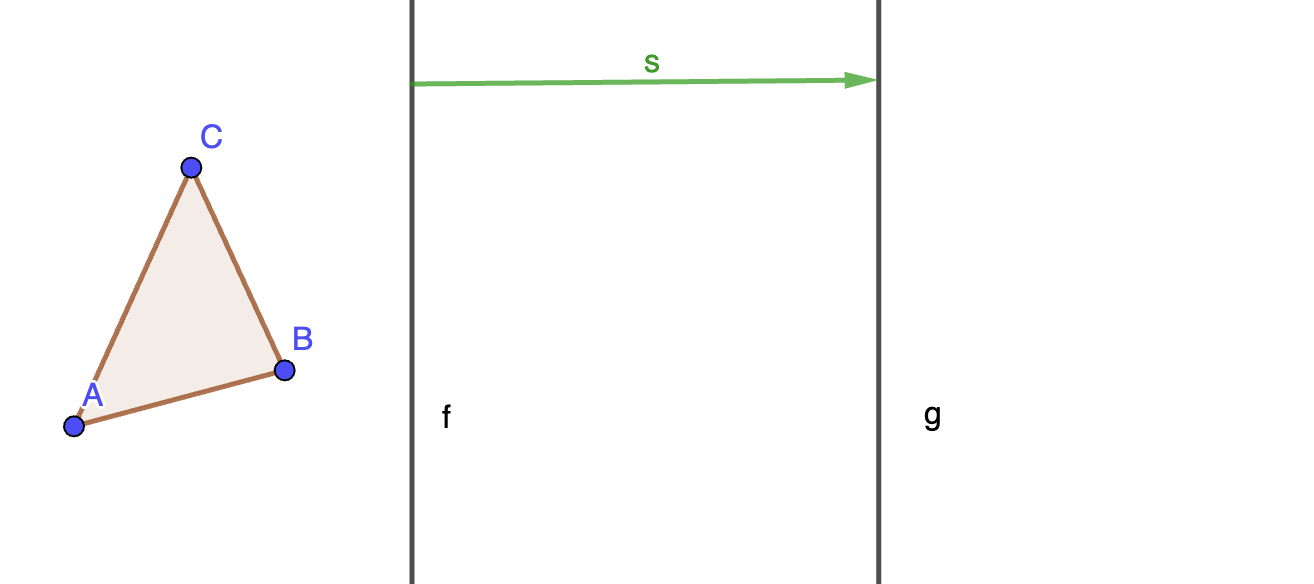
\includegraphics[width=10cm]{zwei-parallele-geraden.png}
\end{center}
\begin{enumerate}[a)]
\item Spiegelt ein allgemeines Dreieck nacheinander an den beiden Geraden in Geogebra. 
\item Verschiebt die Geraden mit festen Abstand $d$ und unter Beibehaltung ihrer Richtung. Was passiert? Könnt ihr euch das erklären?
\item Welche Abbildung ist $f\circ g$? Charakterisiert die Abbildung möglichst genau unter Verwendung von $d$ und der Richtung der Geraden. Begründet, warum es sich um diese Abbildung handelt.
\end{enumerate}

Die Aufgaben orientieren sich an: Krauter, S. \& Bescherer, C. (2013). \emph{Erlebnis Elementargeometrie} (2. Aufl.). Berlin, Heidelberg: Springer. S.~22--26.

\vspace*{10mm}

\printlicense

\printsocials

\end{document}
